% lowell-prop.tex - Lowell Observatory DCT proposal template 
%   Last update 2016-01-04 by hroe@lowell.edu

% General Instructions:
%  
%   Places in the form that require user input are denoted by %%% in this tex
%   file.  Instructions for the sections immediately precede the %%% symbol.
%
%   If you are at a DCT partner institution:
%      - Please fill out at least the cover page portion of this template.
%      - Submit a PDF copy of it to your DCT partner representative, who 
%        will forward it to the DCT Scheduler (tac@lowell.edu)
%
%   Lowell Observatory Users:
%      - Abide by the length limits.
%      - Fill out the cover sheet completely.
%      - Keep in mind that you are writing for a non-specialist audience.
%      - Proposal deadline is listed in the Call for Proposals.
%      - Submit by sending the PDF of your proposal to tac@lowell.edu
%   
%   Questions/comments:  tac@lowell.edu

\documentclass{lowell-prop}

% Uncomment if using figures:
\usepackage{graphicx}

% Uncomment to provide options to siunitx for typesetting units (the class file
% already loads this package and provides the units in http://goo.gl/XzoK8H
% \usepackage[custom-options]{siunitx}
% *Do not* typeset microns as $\mu$m unless you are also expressing kilometers as $k$m.

% Use textgreek to use greek letters which are not math (such as in Hα)
%\usepackage{textgreek}

\begin{document}

% Which telescope(s) are you using?  
% Uncomment one, and only one, of the following lines.
% Note that currently this form is *only* used for DCT, but the following line 
% is here for future compatibility if other facilities are added.
\telescopes{DCT}	% for proposals using DCT only

% Give a descriptive title for the proposal in the \title command.
%
% Note that a title can be quite long; LaTeX will break the title into
% separate lines automatically.  If you wish to indicate line breaks
% yourself, do so with a `\\' command at the appropriate point in
% the title text.
%%%
\title{Mysteries of the universe solved}

% Investigator's (PI and CoI) information blocks.

% Please give the investigator's name, and email address. (The email address of
% the account used to send in the form will be used if you don't fill this in.)
% You must also indicate whether the investigator is a graduate student by
% putting a Y or an N inside the \gradstudent{} curly braces.
%
% Each member of the proposal team is identified with several bits of
% information.
%
%    \name{OBSERVER NAME}
%    \affil{AFFILIATION}
%    \address{POSTAL ADDRESS}
%    \emailaddress{EMAIL ADDRESS}
%    \phone{TELEPHONE NUMBER}
%    \fax{FAX NUMBER}
%    \gradstudent{Y or N}
%    \undergradstudent{Y or N}
%
% Please note that the fax number does not print on the form at this
% time; this is intentional.  We can get your fax number from the
% electronic file if we really have to.
%
% DO NOT remove the \begin{PI} and \end{PI} or the \begin{CoI} and
% \end{CoI} lines.
%
% It is OK to remove unused CoI blocks or add additional CoI blocks as needed.

%%%
\begin{PI}
\name{J. X. Doe}			% REQUIRED
\affiliation{Lowell Observatory}		% REQUIRED
\emailaddress{jxd@lowell.edu}		% REQUIRED
\end{PI}

\begin{CoI}
\name{J. Y. Doe}			% REQUIRED
\affiliation{Lowell Observatory}		% REQUIRED
\emailaddress{jyd@lowell.edu}		% REQUIRED
\end{CoI}

\begin{CoI}
\name{J. Z. Doe}			% REQUIRED
\affiliation{Lowell Observatory}		% REQUIRED
\emailaddress{jzd@lowell.edu}		% REQUIRED
\end{CoI}

\begin{CoI}
\name{J. A. Doe}			% REQUIRED
\affiliation{Lowell Observatory}		% REQUIRED
\emailaddress{jad@lowell.edu}		% REQUIRED
\end{CoI}

\begin{CoI}
\name{J. B. Doe}			% REQUIRED
\affiliation{Lowell Observatory}		% REQUIRED
\emailaddress{jbd@lowell.edu}		% REQUIRED
\end{CoI}


% Give an abstract of the scientific justification.  Please write
% the abstract between the \begin{abstract} and \end{abstract} lines.
% Limit is 100 words.

% DO NOT remove the \begin{abstract} and \end{abstract} lines.

%%%
\begin{abstract}
Lorem ipsum dolor sit amet, consectetur adipiscing elit. Etiam vitae felis lectus. Nulla eu malesuada arcu. Aliquam a arcu in orci semper venenatis sed non purus. Pellentesque tempus nibh dolor. Donec eros lorem, gravida quis euismod eu, tempus sit amet neque. Maecenas tempus ex fermentum purus maximus porttitor. Class aptent taciti sociosqu ad litora torquent per conubia nostra, per inceptos himenaeos. Sed nec metus suscipit metus ultricies fringilla. Pellentesque habitant morbi tristique senectus et netus et malesuada fames ac turpis egestas. Praesent id viverra eros
\end{abstract}



% Indicate whether this proposal is part of your PhD thesis work by
% putting a Y or an N inside the \thesis{} curly braces.  If this is
% thesis work (a "Y" answer), you must attach a copy of your thesis
% prospectus (~1 pages).  Explain in the Scientific Jusification section
% how this proposal is related to your thesis.

%%%
\thesis{N}

% List the details of the observing runs being requested, for
% UP TO THREE runs.  The parameters for each run are segregated
% between \begin{obsrun} and \end{obsrun} lines.  Please be sure
% that the information is isolated properly for each run.
% If the information doesn't quite fit, try preceding it with a
% \small, e.g. \instrument{\small Lengthy description of instrument}
%
%   \telescope{}	For example, \telescope{DCT}
%   \instrument{}	For example, \instrument{LMI: UVBRI, H\textalpha-on,H\textalpha-off; 
%                                                OptiNIRSpec Spectrograph}
%   \numfirsthalfnights{} For exmaple, \numfirsthalfnights{3}
%   \numsecondhalfnights{} For exmaple, \numsecondhalfnights{3}
%   \lunarphase{}	For example, \lunarphase{7}
%   \optimaldates{}	For example, \optimaldates{Sept--Nov}
%   \acceptabledates{}	For example, \acceptabledates{Sept -- mid-Dec}
%   \remoteobserving{}  Either Y or N, if remote observing will be utilized.  
%
% Please select telescope and instrument identifiers from the list...
% Instrument combinations may be specified with "+".
%
% \lunarphase should specify the acceptable number of days from the
% new moon either as:

% 1. a single integer (in which case it will be interpreted
%    symmetrically about the new moon, e.g. 7 == plus or minus seven days
%    from new)
% 2. as two integers (e.g. 7--0, for days before and after the new moon).  
%
% FYI, the tabulated sky brightness with lunar phase is:
%
%                             Table I
%          Sky Brightness as a Function of Lunar Phase
%
% Days from          Sky Brightness (mag/arcsec2)
% New Moon         U       B        V        R       I
%     0          22.0    22.7     21.8     20.9    19.9
%     3          21.5    22.4     21.7     20.8    19.9
%     7          19.9    21.6     21.4     20.6    19.7
%    10          18.5    20.7     20.7     20.3    19.5
%    14          17.0    19.5     20.0     19.9    19.2
%
% (see http://www.noao.edu/noao/noaonews/mar94/art20.html)
%
% \optimaldates should contain the range of OPTIMAL dates (should be
% 2-month window).
%
% \acceptabledates should give the range of ACCEPTABLE dates (i.e., you
% would not accept time outside those limits).

% DO NOT remove the \begin{obsrun} and \end{obsrun} blocks

%%%
\begin{obsrun}
\telescope{DCT}
\instrument{LMI: UVBRI}
\numfirsthalfnights{3}
\numsecondhalfnights{2}
\lunarphase{7--3}
\optimaldates{Feb -- Mar}
\acceptabledates{Jan -- Mar, May-Jun}
\remoteobserving{Y}
\end{obsrun}

\begin{obsrun}	% leave these sections in, even if not used!
\telescope{}
\instrument{}
\numfirsthalfnights{}
\numsecondhalfnights{}
\lunarphase{}
\optimaldates{}
\acceptabledates{}
\remoteobserving{}
\end{obsrun}

\begin{obsrun}
\telescope{}
\instrument{}
\numfirsthalfnights{}
\numsecondhalfnights{}
\lunarphase{}
\optimaldates{}
\acceptabledates{}
\remoteobserving{}
\end{obsrun}

% You may NOT supply more obsrun blocks. Three is the limit. If you need more
% runs, put "More than 3 runs requested" in the instrument section for the THIRD
% run and provide the information for runs 3-N using the following sequence,
% which you should put AFTER the \unusabledates command:
%
% \newpage
% \propsection{\fbox{Additional Runs}} {~} \par
% Some sort of listing of the additional runs. Try using the \tabular environment.

% If there are dates that you cannot use for non-astronomical reasons,
% please give the dates by filling in the curly braces in \unusabledates{}.
% Please explain briefly; \unusabledates is limited to one line.

%%%
\unusabledates{
Sept 24-26, attending conference  Donec euismod egestas ligula ut semper. Pellentesque ultricies metus sit amet laoreet dictum. Pellentesque efficitur leo id orci condimentum lacinia. Vestibulum egestas fermentum dictum. Vestibulum velit lorem, luctus nec sodales eget, rutrum id lorem. In convallis posuere ligula, ac interdum tortor lacinia sit amet. 
%Aenean pulvinar rutrum velit, quis facilisis magna porta a. Praesent et est ac massa posuere lobortis. Proin hendrerit eros ac tincidunt luctus. Maecenas mollis dolor velit, ut iaculis sem efficitur eget. Duis mattis mollis maximus. In vulputate blandit nisl quis pulvinar. Morbi imperdiet ultrices sodales. Nam gravida varius urna, quis dignissim mi dignissim eu. Etiam justo mi, facilisis ac eleifend sagittis, euismod id arcu. Praesent elementum finibus diam, vitae gravida risus lacinia et.
}

% Don't edit or comment out the following line containing \OverflowFromCoverPage{}
% This line will create an additional page if needed to list more CoIs or more observing runs
\OverflowFromCoverPage{}

% In the following "essay question" sections, the delimiting pieces of
% markup (\justification, \feasibility, etc.) act as LaTeX \section*{}
% commands.  If the author wanted to have numbered subsections within
% any of these (as per this sample), LaTeX's \subsection could be used.

% Give the scientific justification for the experiment.
% This section should consist of paragraphs of text (and may include
% figures) that follow the \justification line.
% Be sure to include overall significance to astronomy.

% In order to include a plot, you should use the LaTeX "figure"
% environment with the graphicx package. For example:
%
% \begin{figure}
%     \includegraphics[scale=0.3]{fig} % for fig.pdf, fig.png or fig.eps
%     \caption{Sample Figure showing important results.\label{fig:name}
% \end{figure}

%%%
\justification

Lorem ipsum dolor sit amet, consectetur adipiscing elit. Etiam vitae felis lectus. Nulla eu malesuada arcu. Aliquam a arcu in orci semper venenatis sed non purus. Pellentesque tempus nibh dolor. Donec eros lorem, gravida quis euismod eu, tempus sit amet neque. Maecenas tempus ex fermentum purus maximus porttitor. Class aptent taciti sociosqu ad litora torquent per conubia nostra, per inceptos himenaeos. Sed nec metus suscipit metus ultricies fringilla. Pellentesque habitant morbi tristique senectus et netus et malesuada fames ac turpis egestas. Praesent id viverra eros.

Donec euismod egestas ligula ut semper. Pellentesque ultricies metus sit amet laoreet dictum. Pellentesque efficitur leo id orci condimentum lacinia. Vestibulum egestas fermentum dictum. Vestibulum velit lorem, luctus nec sodales eget, rutrum id lorem. In convallis posuere ligula, ac interdum tortor lacinia sit amet. Aenean pulvinar rutrum velit, quis facilisis magna porta a. Praesent et est ac massa posuere lobortis. Proin hendrerit eros ac tincidunt luctus. Maecenas mollis dolor velit, ut iaculis sem efficitur eget. Duis mattis mollis maximus. In vulputate blandit nisl quis pulvinar. Morbi imperdiet ultrices sodales. Nam gravida varius urna, quis dignissim mi dignissim eu. Etiam justo mi, facilisis ac eleifend sagittis, euismod id arcu. Praesent elementum finibus diam, vitae gravida risus lacinia et.

Morbi mattis non purus at pulvinar. Nullam sollicitudin pretium mi id interdum. Sed eget neque diam. Nam nec arcu at orci luctus efficitur. In a ante rhoncus, scelerisque purus quis, rhoncus nibh. Nunc eget laoreet diam. Integer a fermentum nibh. Fusce luctus fermentum odio, vitae consequat neque fermentum facilisis. Morbi vehicula nec ligula eu rhoncus. Donec in sapien vitae risus condimentum rutrum vel non nisl. Suspendisse potenti. Class aptent taciti sociosqu ad litora torquent per conubia nostra, per inceptos himenaeos. Aliquam imperdiet dignissim neque, in varius lacus dictum aliquet. Ut quis sollicitudin ipsum.

Proin in mollis purus. Nullam erat nunc, elementum nec sollicitudin sed, tincidunt eget sapien. Donec in sem eu odio luctus commodo. Integer accumsan risus ut laoreet vulputate. Aenean quis tempor nunc. Suspendisse pretium ornare vestibulum. Aliquam sollicitudin ac est ac sodales. Ut euismod purus vitae ipsum blandit, vitae semper libero ultrices. Etiam posuere vel dolor ac tempor. Curabitur dapibus pulvinar feugiat. Vivamus nec pellentesque ex. In maximus, nisi congue efficitur tempus, arcu risus eleifend orci, eu facilisis mi sapien non velit. Nam pharetra mollis diam, eu egestas ligula sagittis ac. Cras in nisl accumsan, elementum neque id, aliquet ante. Nam tristique purus sit amet tellus pretium, non fermentum enim dignissim. Nulla facilisis cursus auctor.

Aenean sit amet ornare massa. Integer porta magna aliquet eros tempus, non egestas lorem vehicula. Vivamus sit amet ultrices justo, non euismod nisl. In sed eleifend justo. Sed in purus mi. Sed ac odio imperdiet, tempor elit eget, mollis diam. Phasellus nisl mi, laoreet eu ultrices id, tincidunt quis mauris. In in felis in nisl molestie lacinia vitae eget massa. Nullam tempus lorem velit, eu tincidunt tortor posuere eu. Curabitur malesuada ipsum et maximus lacinia. Donec nibh mauris, lacinia in mi id, vehicula mattis massa. Fusce iaculis in nulla ut luctus. Donec eu eleifend dui. Donec id erat in lacus sodales euismod eu eget augue.

Lorem ipsum dolor sit amet, consectetur adipiscing elit. Etiam vitae felis lectus. Nulla eu malesuada arcu. Aliquam a arcu in orci semper venenatis sed non purus. Pellentesque tempus nibh dolor. Donec eros lorem, gravida quis euismod eu, tempus sit amet neque. Maecenas tempus ex fermentum purus maximus porttitor. Class aptent taciti sociosqu ad litora torquent per conubia nostra, per inceptos himenaeos. Sed nec metus suscipit metus ultricies fringilla. Pellentesque habitant morbi tristique senectus et netus et malesuada fames ac turpis egestas. Praesent id viverra eros.

Donec euismod egestas ligula ut semper. Pellentesque ultricies metus sit amet laoreet dictum. Pellentesque efficitur leo id orci condimentum lacinia. Vestibulum egestas fermentum dictum. Vestibulum velit lorem, luctus nec sodales eget, rutrum id lorem. In convallis posuere ligula, ac interdum tortor lacinia sit amet. Aenean pulvinar rutrum velit, quis facilisis magna porta a. Praesent et est ac massa posuere lobortis. Proin hendrerit eros ac tincidunt luctus. Maecenas mollis dolor velit, ut iaculis sem efficitur eget. Duis mattis mollis maximus. In vulputate blandit nisl quis pulvinar. Morbi imperdiet ultrices sodales. Nam gravida varius urna, quis dignissim mi dignissim eu. Etiam justo mi, facilisis ac eleifend sagittis, euismod id arcu. Praesent elementum finibus diam, vitae gravida risus lacinia et.

Morbi mattis non purus at pulvinar. Nullam sollicitudin pretium mi id interdum. Sed eget neque diam. Nam nec arcu at orci luctus efficitur. In a ante rhoncus, scelerisque purus quis, rhoncus nibh. Nunc eget laoreet diam. Integer a fermentum nibh. Fusce luctus fermentum odio, vitae consequat neque fermentum facilisis. Morbi vehicula nec ligula eu rhoncus. Donec in sapien vitae risus condimentum rutrum vel non nisl. Suspendisse potenti. Class aptent taciti sociosqu ad litora torquent per conubia nostra, per inceptos himenaeos. Aliquam imperdiet dignissim neque, in varius lacus dictum aliquet. Ut quis sollicitudin ipsum.

 \begin{figure}
   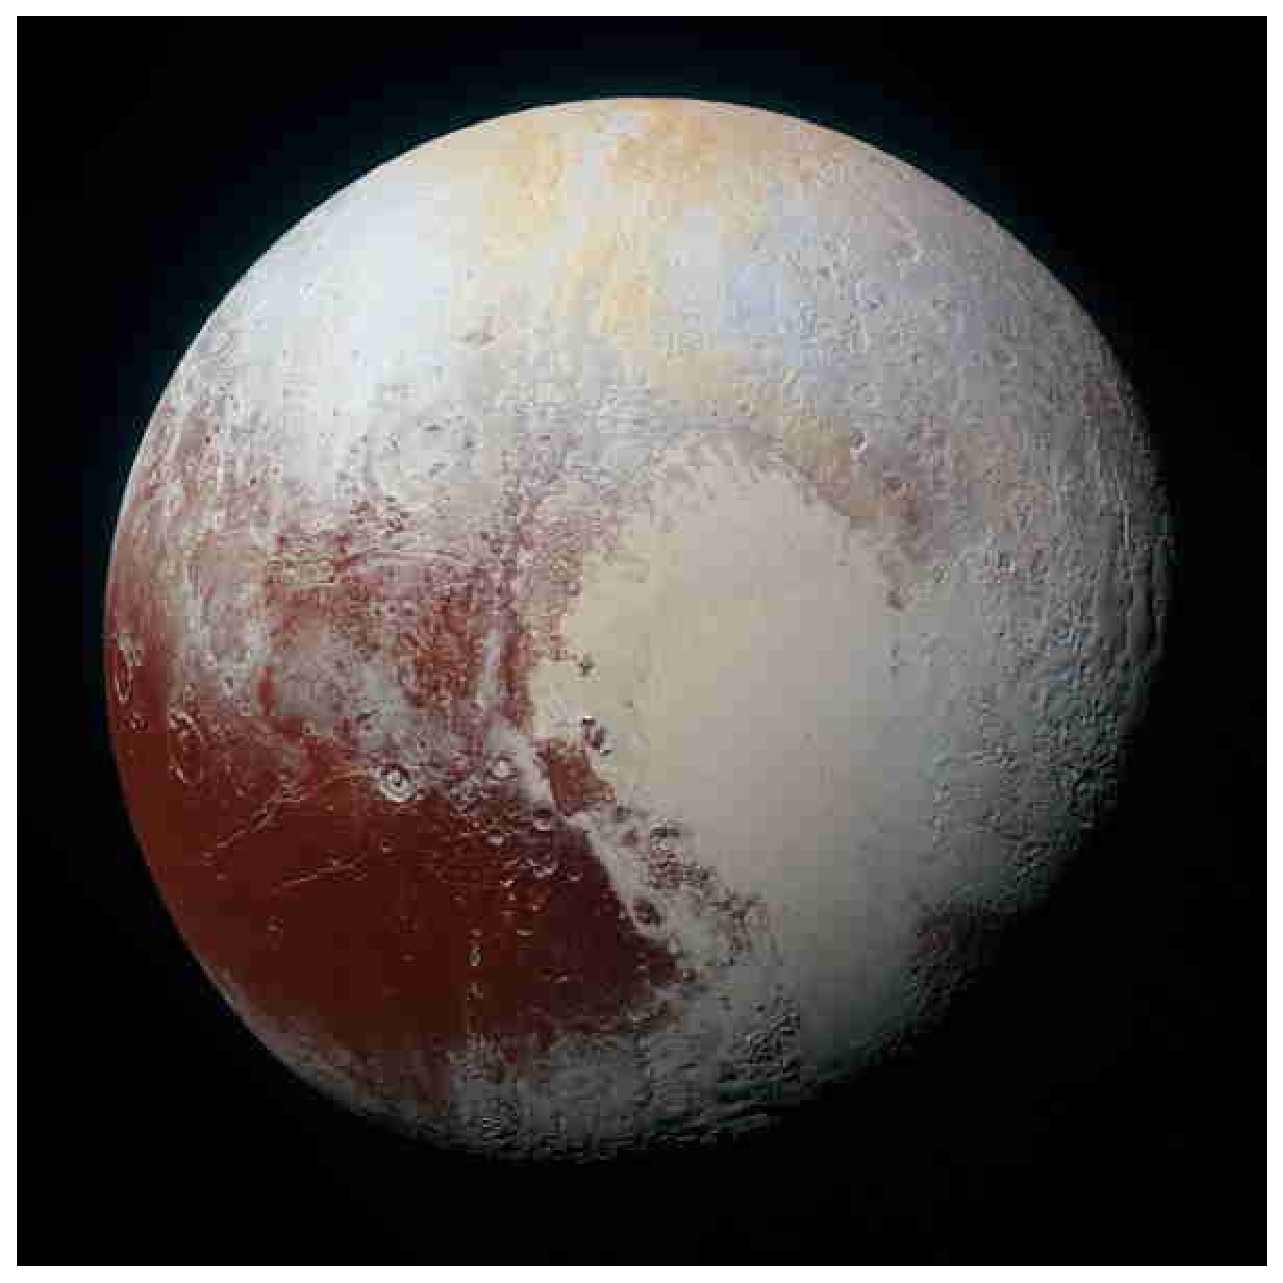
\includegraphics[width=0.5\textwidth]{pluto-small.eps} % for fig.pdf, fig.png or fig.eps
      \caption{Amazing figure to convince the TAC to give me time.}\label{fig:name}
 \end{figure}


Proin in mollis purus. Nullam erat nunc, elementum nec sollicitudin sed, tincidunt eget sapien. Donec in sem eu odio luctus commodo. Integer accumsan risus ut laoreet vulputate. Aenean quis tempor nunc. Suspendisse pretium ornare vestibulum. Aliquam sollicitudin ac est ac sodales. Ut euismod purus vitae ipsum blandit, vitae semper libero ultrices. Etiam posuere vel dolor ac tempor. Curabitur dapibus pulvinar feugiat. Vivamus nec pellentesque ex. In maximus, nisi congue efficitur tempus, arcu risus eleifend orci, eu facilisis mi sapien non velit. Nam pharetra mollis diam, eu egestas ligula sagittis ac. Cras in nisl accumsan, elementum neque id, aliquet ante. Nam tristique purus sit amet tellus pretium, non fermentum enim dignissim. Nulla facilisis cursus auctor.

Aenean sit amet ornare massa. Integer porta magna aliquet eros tempus, non egestas lorem vehicula. Vivamus sit amet ultrices justo, non euismod nisl. In sed eleifend justo. Sed in purus mi. Sed ac odio imperdiet, tempor elit eget, mollis diam. Phasellus nisl mi, laoreet eu ultrices id, tincidunt quis mauris. In in felis in nisl molestie lacinia vitae eget massa. Nullam tempus lorem velit, eu tincidunt tortor posuere eu. Curabitur malesuada ipsum et maximus lacinia. Donec nibh mauris, lacinia in mi id, vehicula mattis massa. Fusce iaculis in nulla ut luctus. Donec eu eleifend dui. Donec id erat in lacus sodales euismod eu eget augue.


% Assess the technical and scientific feasibility of the experiment.
% This section should consist of paragraphs of text only (no figures)
% that follow the \feasibility line.
%
% List objects, coordinates, and magnitudes (or surface brightness,
% if appropriate), desired S/N, wavelength coverage and resolution.
% Justify the number of nights requested as well as the specific
% telescope(s), instruments, and lunar phase. If you've requested
% long-term status, explain why this is necessary for successful
% completion of the science.  

%%%
\feasibility 

Proin in mollis purus. Nullam erat nunc, elementum nec sollicitudin sed, tincidunt eget sapien. Donec in sem eu odio luctus commodo. Integer accumsan risus ut laoreet vulputate. Aenean quis tempor nunc. Suspendisse pretium ornare vestibulum. Aliquam sollicitudin ac est ac sodales. Ut euismod purus vitae ipsum blandit, vitae semper libero ultrices. Etiam posuere vel dolor ac tempor. Curabitur dapibus pulvinar feugiat. Vivamus nec pellentesque ex. In maximus, nisi congue efficitur tempus, arcu risus eleifend orci, eu facilisis mi sapien non velit. Nam pharetra mollis diam, eu egestas ligula sagittis ac. Cras in nisl accumsan, elementum neque id, aliquet ante. Nam tristique purus sit amet tellus pretium, non fermentum enim dignissim. Nulla facilisis cursus auctor.

Aenean sit amet ornare massa. Integer porta magna aliquet eros tempus, non egestas lorem vehicula. Vivamus sit amet ultrices justo, non euismod nisl. In sed eleifend justo. Sed in purus mi. Sed ac odio imperdiet, tempor elit eget, mollis diam. Phasellus nisl mi, laoreet eu ultrices id, tincidunt quis mauris. In in felis in nisl molestie lacinia vitae eget massa. Nullam tempus lorem velit, eu tincidunt tortor posuere eu. Curabitur malesuada ipsum et maximus lacinia. Donec nibh mauris, lacinia in mi id, vehicula mattis massa. Fusce iaculis in nulla ut luctus. Donec eu eleifend dui. Donec id erat in lacus sodales euismod eu eget augue.

% How effectively have you used DCT and other related telescope time
% in the past?  List your allocation of telescope time at DCT during the past 2 years,
% together with the current status of the data (cite publications
% where appropriate).  Mark any allocations of time related to the
% current proposal with a \relatedwork{} command.  If you have
% requested remote observing in any of your runs, indicate here
% the on-site prior experience with the relevant instrument(s).

%%%
\thepast
November 2015, 2n DCT, "Looking for liners in all the wrong places"  

%\relatedwork{}

\end{document}

